\chapter{Documentação de Funções}
\label{ch::doc-codigo}

% \section{Funções MATLAB Transcritas para Python}
% \label{sec::doc-codigo:transcrito}

% \chapter{Documentação de Funções MATLAB Transcritas para Python}
% \label{ch::doc-codigo-transcrito}

\section{Função \texttt{load\_hologram}}
\label{sec::doc-codigo:load_hologram}

\begin{table}[!hp]
    \centering
    \caption{Documentação da função \texttt{load\_hologram}.}
    \label{tab:load_hologram}
    \begin{tabular}{p{1cm} p{11.5cm}}
        \hline
        \multicolumn{2}{l}{\bfseries\small Nome da função}\\
         & \verb|load_hologram|\\
        \hline
        \multicolumn{2}{l}{\bfseries\small Protótipo original em MATLAB}\\
         & \mintinline[breaklines]{matlab}{function [hologram] = load_hologram(ampli_path, phase_path)}\\
        \hline
        \multicolumn{2}{l}{\bfseries\small Protótipo transcrito em Python}\\
         & \mintinline{python}{def load_hologram(ampli_path, phase_path)} \\
        \hline\multicolumn{2}{l}{\bfseries\small Descrição}\\
         & Esta função carrega um holograma da base de dados b<>com a partir dos seus ficheiros de amplitude e fase.\\
        \hline\multicolumn{2}{l}{\bfseries\small \textit{Inputs}}\\
         & \verb|ampli_path|: Diretório do ficheiro da imagem da amplitude (caminho relativo ou absoluto).\\
         & \verb|phase_path|: Diretório do ficheiro da imagem da fase (caminho relativo ou absoluto).\\
        \hline\multicolumn{2}{l}{\bfseries\small \textit{Output}}\\
         & Modulação complexa do holograma (3 canais: \ac{RGB}).\\
        \hline\multicolumn{2}{l}{\bfseries\small Efeitos colaterais}\\
         & Não aplicável. \\
        \hline\multicolumn{2}{l}{\bfseries\small Dependências}\\
         & Não aplicável. \\
        \hline
    \end{tabular}
\end{table}


\newpage
\section{Função \texttt{propagate\_asm}}
\label{sec::doc-codigo:propagate_asm}

\begin{table}[!hp]
    \centering
    \caption{Documentação da função \texttt{propagate\_asm}.}
    \label{tab:propagate_asm}
    \begin{tabular}{p{1cm} p{11.5cm}}
        \hline
        \multicolumn{2}{l}{\bfseries\small Nome da função}\\
         & \verb|propagate_asm|\\
        \hline
        \multicolumn{2}{l}{\bfseries\small Protótipo original em MATLAB}\\
         & \mintinline[breaklines]{matlab}{function [v] = propagate_asm(u, pitch, wavelength, z)}\\
        \hline
        \multicolumn{2}{l}{\bfseries\small Protótipo transcrito em Python}\\
         & \mintinline[breaklines]{python}{def propagate_asm(u, pitch, wavelength, z)} \\
        \hline\multicolumn{2}{l}{\bfseries\small Descrição}\\
         & Esta função simula a propagação no plano complexo \verb|u| sobre a distância \verb|z| utilizando o \ac{ASM}.\\
        \hline\multicolumn{2}{l}{\bfseries\small \textit{Inputs}}\\
         & \verb|u|: Campo de onda de luz do plano de \textit{input} (um canal).\\
         & \verb|pitch|: Distância entre pixeis (em metros).\\
         & \verb|wavelength|: Comprimento de onda do canal de cor a propagar (em metros).\\
         & \verb|z|: Distância de propagação ao longo do eixo ótico (em metros).\\
        \hline\multicolumn{2}{l}{\bfseries\small \textit{Output}}\\
         & Campo de onda de luz no plano de destino (um canal).\\
        \hline\multicolumn{2}{l}{\bfseries\small Efeitos colaterais}\\
         & Não aplicável. \\
        \hline\multicolumn{2}{l}{\bfseries\small Dependências}\\
         & Não aplicável. \\
        \hline
    \end{tabular}
\end{table}


\newpage
\section{Função \texttt{reconst\_hologram}}
\label{sec::doc-codigo:reconst_hologram}

\begin{table}[!hp]
    \centering
    \caption{Documentação da função \texttt{reconst\_hologram}.}
    \label{tab:reconst_hologram}
    \begin{tabular}{p{1cm} p{11.5cm}}
        \hline
        \multicolumn{2}{l}{\bfseries\small Nome da função}\\
         & \verb|reconst_hologram|\\
        \hline
        \multicolumn{2}{l}{\bfseries\small Protótipo original em MATLAB}\\
         & \mintinline[breaklines]{matlab}{function [recons] = reconsHologram(hologram, pitch, wavelengths, z, pupilPos, pupilSize)
         }\\
        \hline
        \multicolumn{2}{l}{\bfseries\small Protótipo transcrito em Python}\\
         & \mintinline[breaklines]{python}{def reconst_hologram(hologram, pitch, wavelengths, z, pupil_pos, pupil_size)} \\
        \hline\multicolumn{2}{l}{\bfseries\small Descrição}\\
         & Esta função reconstrói o holograma a uma distância \verb|z|, utilizando o \ac{ASM}. Permite o uso de uma janela para obter reconstruções de diferentes pontos de vista.\\
        \hline\multicolumn{2}{l}{\bfseries\small \textit{Inputs}}\\
         & \verb|hologram|: Holograma de modulação complexa (3 canais: \ac{RGB}). \\
         & \verb|pitch|: Distância entre pixeis (em metros).\\
         & \verb|wavelengths|: Comprimentos de onda de luz (em metros, 3 canais: \ac{RGB}).\\
         & \verb|z|: Distância de reconstrução (em metros).\\
         & \verb|pupilPos|: Posição da janela (em pixeis, canto superior direito).\\
         & \hspace{1cm} \textit{Valor por defeito.} \verb|[0, 0]|.\\
         & \verb|pupilSize|: Tamanho da janela (em pixeis, altura $\times$ largura).\\
         & \hspace{1cm} \textit{Valor por defeito.} \verb|None|.\\
        \hline\multicolumn{2}{l}{\bfseries\small \textit{Output}}\\
         & Reconstrução numérica do holograma (3 canais: \ac{RGB}).\\
        \hline\multicolumn{2}{l}{\bfseries\small Efeitos colaterais}\\
         & Não aplicável. \\
        \hline\multicolumn{2}{l}{\bfseries\small Dependências}\\
         & Função \verb|propagate_asm| (Tabela \ref{tab:propagate_asm}). \\
        \hline
    \end{tabular}
\end{table}


% \chapter{Documentação de Funções para Reconstrução de Hologramas em Multivista}
% \label{ch::doc-codigo-reconst}

\newpage
\section{Função \texttt{reconst\_16views}}
\label{sec::doc-codigo:reconst_16views}

\begin{table}[!hp]
    \centering
    \caption{Documentação da função \texttt{reconst\_16views}.}
    \label{tab:reconst_16views}
    \begin{tabular}{p{1cm} p{11.5cm}}
        \hline
        \multicolumn{2}{l}{\bfseries\small Nome da função}\\
         & \verb|reconst_16views|\\
        \hline
        \multicolumn{2}{l}{\bfseries\small Protótipo em Python}\\
         & \mintinline[breaklines]{python}{def reconst_16views(hologram)} \\
        \hline\multicolumn{2}{l}{\bfseries\small Descrição}\\
         & Reconstrói o holograma fornecido por argumento em 16 vistas. \\
         & \textit{Processo.} Carrega o holograma (dois ficheiros \textit{bitmap}: amplitude e fase) e o respetivo ficheiro de especificações (formato \ac{JSON}). Calcula as posições das 16 vistas tendo em conta o tamanho do holograma.\\
        \hline\multicolumn{2}{l}{\bfseries\small \textit{Inputs}}\\
         & \verb|hologram|: Nome do holograma a ser reconstruído.\\
         & \hspace{1cm} \textit{Valor por defeito.} ``\verb|dices4k|''.\\
        \hline\multicolumn{2}{l}{\bfseries\small \textit{Output}}\\
         & Não aplicável.\\
        \hline\multicolumn{2}{l}{\bfseries\small Efeitos colaterais}\\
         & Produz, dentro da pasta \verb|./reconst/|, uma nova pasta com o nome do holograma. O respetivo conteúdo incluirá as 16 vistas (ficheiros \verb|*.ppm|) correspondentes às reconstruções produzidas pela função.\\
        \hline\multicolumn{2}{l}{\bfseries\small Dependências}\\
         & Função \verb|load_hologram| (Tabela \ref{tab:load_hologram}); \\
         & Função \verb|reconst_hologram| (Tabela \ref{tab:reconst_hologram}). \\
         & \textit{Ver Figura \ref{fig:reconst_16views}.} \\
        \hline
    \end{tabular}
\end{table}

\begin{figure}[!hp]
    \centering
    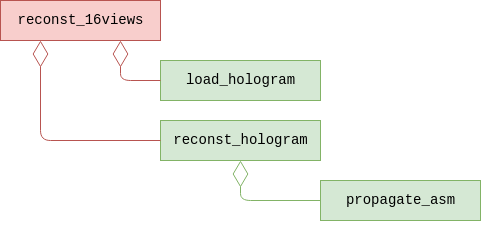
\includegraphics[scale=.6]{reconst_16views}
    \caption{Diagrama de dependências da função \texttt{reconst\_16views}.}
    \label{fig:reconst_16views}
\end{figure}

% \chapter{Documentação de Funções para Compressão e Descompressão de Hologramas Reconstruídos}
% \label{ch::doc-codigo-compress}

\newpage
\section{Função \texttt{compress\_views}}
\label{sec::doc-codigo:compress_views}

\begin{table}[!hp]
    \centering
    \caption{Documentação da função \texttt{compress\_views}.}
    \label{tab:compress_views}
    \begin{tabular}{p{1cm} p{11.5cm}}
        \hline
        \multicolumn{2}{l}{\bfseries\small Nome da função}\\
         & \verb|compress_views|\\
        \hline
        \multicolumn{2}{l}{\bfseries\small Protótipo em Python}\\
         & \mintinline[breaklines]{python}{def compress_views(hologram, ycbcr, rate)} \\
        \hline\multicolumn{2}{l}{\bfseries\small Descrição}\\
         & Comprimir os hologramas e calcular o \ac{PSNR}. \\
         & \textit{Processo.} Para cada vista, o holograma é codificado, descodificado e analisado em termos do \ac{PSNR}. São criados 16 ficheiros \verb|*.jp2| por pasta \verb|rate_n|, correspondentes às 16 vistas reconstruídas, assim como ficheiros \ac{JSON} (um por holograma) na pasta \verb|kduOutput| com as métricas de compressão (\ac{PSNR}). \\
        \hline\multicolumn{2}{l}{\bfseries\small \textit{Inputs}}\\
         & \verb|hologram|: Nome do holograma a comprimir.\\
         & \hspace{1cm} \textit{Valor por defeito.} ``\verb|dices4k|''.\\
         & \verb|ycbcr|: \textit{Flag} que indica ao \ac{kdu} se deve ser efetuada uma transformada de cor.\\
         & \hspace{1cm} \textit{Valor por defeito.} \verb|False|.\\
         & \verb|rate|: número de \textit{bits} por amostra.\\
         & \hspace{1cm} \textit{Valor por defeito.} \verb|1.0|.\\
        \hline\multicolumn{2}{l}{\bfseries\small \textit{Output}}\\
         & Não aplicável.\\
        \hline\multicolumn{2}{l}{\bfseries\small Efeitos colaterais}\\
         & Armazena as imagens no formato \verb|*.jp2| nas pastas \verb|rate_n|, assim como os ficheiros \ac{JSON} na pasta \verb|kduOutput|, segundo a seguinte árvore de diretórios:\\
         & \dirtree{%
            .1 ./kduOutput.
            % .2 dices4k.
            .2 <nome\_holograma>.
            .3 no\_ycbcr.
            .4 rate\_n\DTcomment{\small $n$: número de \textit{bits}}.
            % .4 \ldots.
            .3 ycbcr.
            % .2 diffuseCar4k\DTcomment{\textit{idem}}.
            % .2 piano4k.
         } \\
        \hline\multicolumn{2}{l}{\bfseries\small Dependências}\\
        & Função \verb|cod_jpeg2000| (Tabela \ref{tab:cod_jpeg2000});\\
        & Função \verb|dec_jpeg2000| (Tabela \ref{tab:dec_jpeg2000});\\
        & Função \verb|psnr| (Tabela \ref{tab:psnr}).\\
        & \textit{Ver Figura \ref{fig:compress_views}.} \\
        \hline
    \end{tabular}
\end{table}

\begin{figure}[!hp]
    \centering
    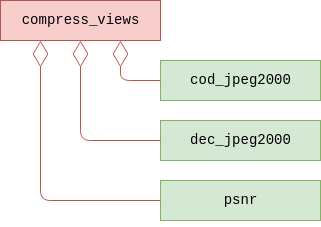
\includegraphics[scale=.6]{compress_views}
    \caption{Diagrama de dependências da função \texttt{compress\_views}.}
    \label{fig:compress_views}
\end{figure}

\newpage
\section{Função \texttt{cod\_jpeg2000}}
\label{sec::doc-codigo:cod_jpeg2000}

\begin{table}[!hp]
    \centering
    \caption{Documentação da função \texttt{cod\_jpeg2000}.}
    \label{tab:cod_jpeg2000}
    \begin{tabular}{p{1cm} p{11.5cm}}
        \hline
        \multicolumn{2}{l}{\bfseries\small Nome da função}\\
         & \verb|cod_jpeg2000|\\
        \hline
        \multicolumn{2}{l}{\bfseries\small Protótipo em Python}\\
         & \mintinline[breaklines]{python}{def cod_jpeg2000(in_path, out_path, ycbcr, rate)} \\
        \hline\multicolumn{2}{l}{\bfseries\small Descrição}\\
         & Invoca ao sistema a execução do comando \verb|kdu_compress|, conforme descrito na Secção \ref{ssec::tecno-ferr:tecno-ferr:kdu}. \\
        \hline\multicolumn{2}{l}{\bfseries\small \textit{Inputs}}\\
         & \verb|in_path|: caminho do ficheiro de \textit{input}. \\
         & \verb|out_path|: caminho do ficheiro de \textit{output}. \\
         & \hspace{1cm} \textit{Valor por defeito.} ``\verb|out.jp2|''.\\
         & \verb|ycbcr|: \textit{flag} que indica ao \ac{kdu} se deve ser efetuada uma transformada de cor. \\
         & \hspace{1cm} \textit{Valor por defeito.} \verb|False|.\\
         & \verb|rate|: número de \textit{bits} por amostra. \\
         & \hspace{1cm} \textit{Valor por defeito.} \verb|1.0|.\\
        \hline\multicolumn{2}{l}{\bfseries\small \textit{Output}}\\
         & Não aplicável. \\
        \hline\multicolumn{2}{l}{\bfseries\small Efeitos colaterais}\\
         & Gera uma imagem no formato \verb|*.jp2| no diretório definido por \verb|out_path|. \\
        \hline\multicolumn{2}{l}{\bfseries\small Dependências}\\
         & Não aplicável. \\
        \hline
    \end{tabular}
\end{table}


\newpage
\section{Função \texttt{dec\_jpeg2000}}
\label{sec::doc-codigo:dec_jpeg2000}

\begin{table}[!hp]
    \centering
    \caption{Documentação da função \texttt{dec\_jpeg2000}.}
    \label{tab:dec_jpeg2000}
    \begin{tabular}{p{1cm} p{11.5cm}}
        \hline
        \multicolumn{2}{l}{\bfseries\small Nome da função}\\
         & \verb|dec_jpeg2000|\\
        \hline
        \multicolumn{2}{l}{\bfseries\small Protótipo em Python}\\
         & \mintinline[breaklines]{python}{def dec_jpeg2000(in_path, out_path, ycbcr, rate)} \\
        \hline\multicolumn{2}{l}{\bfseries\small Descrição}\\
         & Invoca ao sistema a execução do comando \verb|kdu_expand|, conforme descrito na Secção \ref{ssec::tecno-ferr:tecno-ferr:kdu}. \\
        \hline\multicolumn{2}{l}{\bfseries\small \textit{Inputs}}\\
         & \verb|in_path|: caminho do ficheiro de \textit{input}. \\
         & \verb|out_path|: caminho do ficheiro de \textit{output}. \\
         & \hspace{1cm} \textit{Valor por defeito.} ``\verb|out.jp2|''.\\
         & \verb|ycbcr|: \textit{flag} que indica ao \ac{kdu} se deve ser efetuada uma transformada de cor. \\
         & \hspace{1cm} \textit{Valor por defeito.} \verb|False|.\\
         & \verb|rate|: número de \textit{bits} por amostra. \\
         & \hspace{1cm} \textit{Valor por defeito.} \verb|1.0|.\\
        \hline\multicolumn{2}{l}{\bfseries\small \textit{Output}}\\
         & Não aplicável. \\
        \hline\multicolumn{2}{l}{\bfseries\small Efeitos colaterais}\\
         & Gera uma imagem no formato \verb|*.tmp| no diretório definido por \verb|out_path|. \\
        \hline\multicolumn{2}{l}{\bfseries\small Dependências}\\
         & Não aplicável. \\
        \hline
    \end{tabular}
\end{table}


% \chapter{Documentação de Funções para Cálculo das Métricas de Compressão}
% \label{ch::doc-codigo-psnr}

\newpage
\section{Função \texttt{psnr}}
\label{sec::doc-codigo:psnr}

\begin{table}[!hp]
    \centering
    \caption{Documentação da função \texttt{psnr}.}
    \label{tab:psnr}
    \begin{tabular}{p{1cm} p{11.5cm}}
        \hline
        \multicolumn{2}{l}{\bfseries\small Nome da função}\\
         & \verb|psnr|\\
        \hline
        \multicolumn{2}{l}{\bfseries\small Protótipo em Python}\\
         & \mintinline[breaklines]{python}{def psnr(p1, p2)} \\
        \hline\multicolumn{2}{l}{\bfseries\small Descrição}\\
         & Calcula a métrica de compressão \ac{PSNR} entre duas imagens. \\
        \hline\multicolumn{2}{l}{\bfseries\small \textit{Inputs}}\\
         & \verb|p1|: caminho para a primeira imagem. \\
         & \verb|p2|: caminho para a segunda imagem. \\
        \hline\multicolumn{2}{l}{\bfseries\small \textit{Output}}\\
         & Valor calculado do \ac{PSNR}. \\
        \hline\multicolumn{2}{l}{\bfseries\small Efeitos colaterais}\\
         & Não aplicável. \\
        \hline\multicolumn{2}{l}{\bfseries\small Dependências}\\
         & Não aplicável. \\
        \hline
    \end{tabular}
\end{table}
